%参考:https://tex.stackexchange.com/questions/255234/how-does-one-pick-control-points-to-control-b%C3%A9zier-curves-in-tikz

\documentclass[border=5]{standalone}

\usepackage{tikz}
\usetikzlibrary{decorations.pathreplacing}

\tikzset{%
  show curve controls/.style={
    postaction={
      decoration={
        show path construction,
        curveto code={
          \draw [blue] 
            (\tikzinputsegmentfirst) -- (\tikzinputsegmentsupporta)
            (\tikzinputsegmentlast) -- (\tikzinputsegmentsupportb);
          \fill [red, opacity=0.5] 
            (\tikzinputsegmentsupporta) circle [radius=.5ex]
            (\tikzinputsegmentsupportb) circle [radius=.5ex];
        }
      },
      decorate
}}}

\begin{document}
	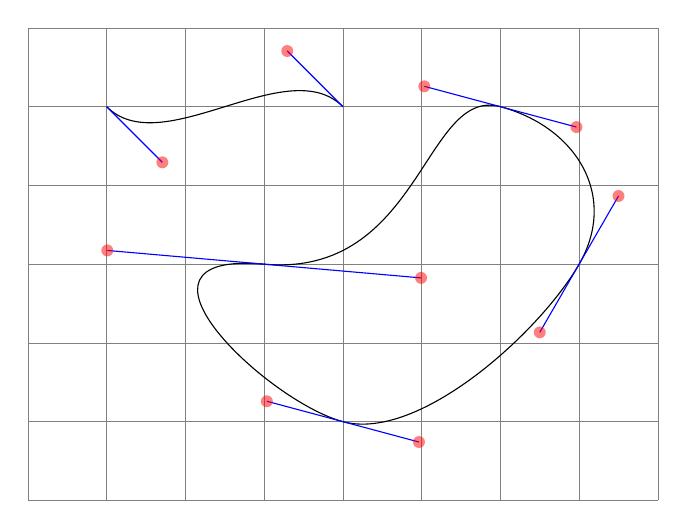
\begin{tikzpicture}
		\draw [help lines] (-4, -1) grid (4, 5);
		\draw [show curve controls]
		  (-3, 4) .. controls ++(135:-1) and ++(135:1) .. (0, 4);
		\draw [show curve controls] (0, 0) 
		  .. controls ++(165:-1) and ++(240: 1) .. ( 3, 2)
		  .. controls ++(240:-1) and ++(165:-1) .. ( 2, 4)
		  .. controls ++(165: 1) and ++(175:-2) .. (-1, 2)
		  .. controls ++(175: 2) and ++(165: 1) .. ( 0, 0);
	\end{tikzpicture}
\end{document}